\chapter{Random Walks}
In this chapter we will consider the concept of Random Walks and also 
the evolution provided by \emph{pagerank} (invented in $1997$ by Google)
in ranking document.

Given a graph of nodes, like nodes in web graph, we use the adjacency matrix
$A$ which has $a_{ij} = 0$ if not exist a edge from $i$ to $j$ otherwise 
has value $1$.\newline
From adjacency matrix we define the transition matrix $P$, which estabilish
a weight to each edge of a graph $G$ and has as constraints that every row
in the transition matrix $P$ has to sum to $1$; in figure \ref{img:transition}
is possible to see how are defined adjacency and transition matrix for a graph,
note anyway that transition matrix is not unique.

\begin{figure}
	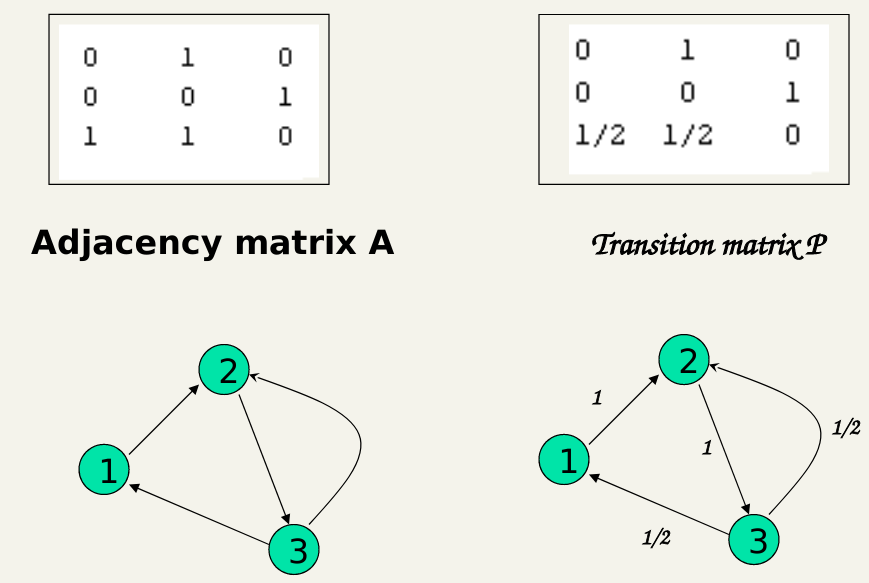
\includegraphics[width=\textwidth]{Images/transition}
	\caption{Transition matrix for a graph $G$}
	\label{img:transition}
\end{figure}
A random walk consist a random walk in the graph starting from an arbitrary
node using $t$ movement in the graph, we define the probability to be 
in a node $i$ at time $t$ as $x_t(i)$ and we update the position from time
$t$ to time $t + 1$ as 
\[ x_{t + 1}(i) = \sum _j x_t(j) * P(j, i) = x_t * P \]

Defined in that way we can obtain a recursive definition of $x_{t+1}$ as 
\[ x_{t+1} = x_t * P = (x_{t-1} * P) * P = \dots = x_0 P^{t+1} \]
If we have that the surfer keeps the same position for a long time we have
the called \emph{stationary distribution}.\newline
This distribution is related to the amound of time that a random walker
spends visiting that node and formaly is defined as 
\[ x_{t+1} = x_t \]
that corrispond to left eigenvector, with eigenvalue $1$ and for 
"well-behaved" graphs this does not depend on the start distribution $x_0$.

The stationary distribution always exist and it is unique if the graph 
(called also \emph{markov chain}) is irreducible and aperiodic, where
irreducible means that there is a path from every node to every other node
and it is aperiodic if the GCD of all cycle lengths is $1$.

\section{Link-based Ranking and Pagerank}
We view the web as a directed graph, where we have $2$ assumptions:
\begin{enumerate}
   \item A hyperlink between pages denotes author perceived relevance
	 (quality signal).
   \item The text in the anchor of the hyperlink describes the target page
	 (textual context).
\end{enumerate}


In first generation of search engine it was used link counts as simple
measures of popularity, but these approach is easy to spam, so to solve
this problem in $1997$ Google introduce \emph{Pagerank}, where each link
has its own importance and it is independent of the query.\newline
Pagerank can be viewed as a linear system of equations with billion variables
and billion contraints or also as a random walk on the Web graph, as can
be viewed in figure \ref{img:pagerank} where $\alpha = 0.85$ as google 
in the original paper estabilish.

\begin{figure}
	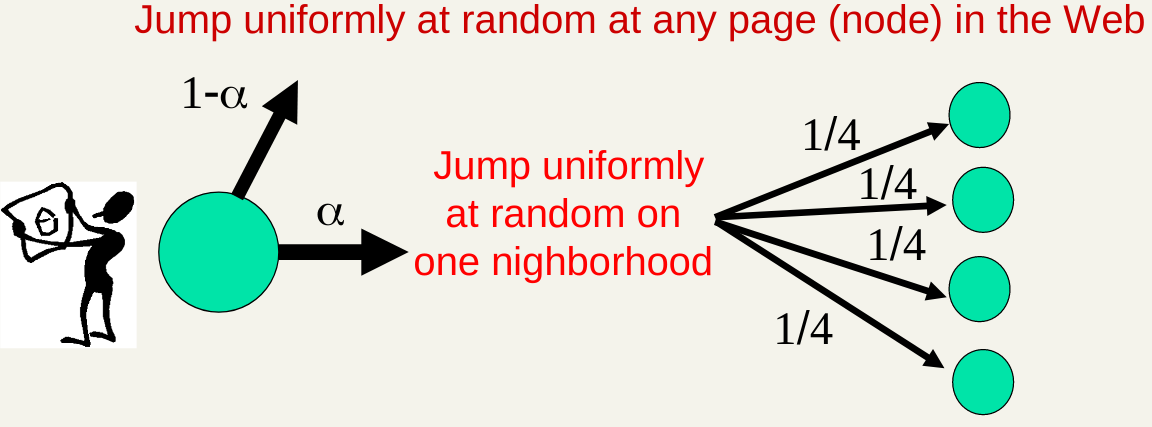
\includegraphics[width=\textwidth]{Images/pagerank}
	\caption{Pagerank approach on a node}
	\label{img:pagerank}
\end{figure}
Pagerank of a node is the "frequency of visit" that node by assuming an
infinite random walk and is a "measure of centrality"
of a node in a directed graph.

View a Pagerank as a linear system of equations we define the pagerank as 
\[ r(i) = \alpha * \sum _{j \in B(i)} \frac{r(j)}{\# out(j)} + 
	  (1 - \alpha) * \frac{1}{N} \]
where $\alpha = 0.85$ and $N = \#$ nodes in graph.\newline
This definition is related to the eigenvalues of the matrix 
describing the linear system of equations.

Pagerank is used in search engines in preprocessing, where given graph we
build $P$ and we compute $r = [1/N, \dots, 1/N] * P^t$, and also in 
query processing, where we retrieve pages containing query terms and 
rank them by their Pagerank.

Relevance is a not well defined mathematical concept, which is actually not 
even depending on the single user because its needs may change over time too,
so for every page search engine computes a series of features (TF-IDF, Pagerank,
occurency in URL, occurrence in the title and so on) and to rank we have
a strong use of AI and Machine Learning, using a classifier.

An evolution of Pagerank is the \emph{Personalized Pagerank}, where we bias
the random jump substituting the uniform jump to all nodes with the jump to
one specific node, which the second term is $(1 - \alpha)$ only for that node
and in the others are $0$, or a uniform jump to some set $S$ of preferred
nodes (is a generalization of the first with $|S| = 1$); it can also be 
not a uniform jump using proper weight in the definition of $r$ and the 
equation for Pagerank of a node in this personalizated version is 
\[ r(i) = \begin{cases}
	\alpha * \sum _{j \in B(i)} \frac{r(j)}{\# out(j)} + (1 - \alpha) * \frac{1}{N} \, \text{ if } i \text{ is teh personalize node } \\
	\alpha * \sum _{j \in B(i)} \frac{r(j)}{\# out(j)} \, \text{otherwise} \\
	  \end{cases} \]

\section{HITS (Hypertext Induced Topic Search}
In this section we will consider another ranking approach that has some 
pitfalls that denies his use in web engine, but are sometimes used in 
private information retrieval system.

Hits, with a common graph architecture visible in figure \ref{img:hits},
is query-dependent and produces two scores per page:
\begin{description}
    \item [Authority score:] a good authority page for a topic is pointed
	   to by many good hubs for that topic.
    \item [Hub score:] a good hub page for a topic points to many authorative
	    pages for that topic.
\end{description}

\begin{figure}
	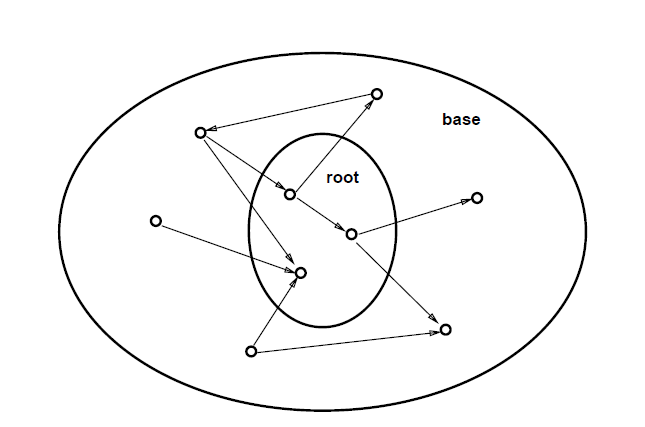
\includegraphics[width=\textwidth]{Images/hits}
	\caption{Hits Graph architecture}
	\label{img:hits}
\end{figure}
To compute this score we have the following equations:
\begin{align*}
	a & = \transpose{A} h = \transpose{A} Aa \\
	h & = Aa = A \transpose{A} h \\
\end{align*}
where $a$ is the vector of authority's scores, $h$ is the vector of 
hub's scores and $A$ is the adjacency matrix, so we have that $h$ is an
eigenvector of $A \transpose{A}$ and $a$ is an eigenvector of $\transpose{A} A$.

We can have link with weight, so we weight more if the query occurs in the
neighborhood of the link and then we define the following equations
\begin{align*}
	h(x) & = \sum _{x \to y} w(x, y) a(y) \\
	a(x) & = \sum _{y \to x} w(x, y) h(y) \\
\end{align*}
The simple idea of rank via random walks consist to rank and select
sentences by saliency score of their constituting words $w$ computed using:
\begin{itemize}
    \item TF-IDF for weight $w$ using the formula
	    \[ saliency(S_i) = \sum _{w \in S_i} \frac{weight(w)}{|S_i|} \]
    \item Centrality over proper graphs: Pagerank, HITS, or other measures.
\end{itemize}

We introduce \emph{TextRank}, where the key issue of this approach is that 
the graph has as nodes terms or sentences and as edges the similarity 
relation between nodes defined as 
\[ Similarity(S_i, S_j) = \frac{|S_i \cap S_j}{\log |S_i| + \log |S_j|} \]
It use Pagerank over weighted graph and compute the score of nodes.

Another ranked that we will introduce is the \emph{lexical Pagerank}, which
the main difference with TextRank resides in the way it is computed 
edge weigts: it use cosine similarity via TF-IDF between sentences and 
edges are pruned if weight $<$ threshold.\newline
The scoring of nodes is done via weighted HITS to ensure mutual reinforcement
between words and sentences.

\section{LSI (Latent Semantic Indexing)}
In this section we will analyze how to reduce dimension of vector while 
we preserve distance, so to compute $cos(d, q)$ for all $n$ docs we can 
reduce the time complexity from $O(nm)$ to $O(km + kn)$ where $k << n, m$.

Instead Random projection is data-independent and consist to choose a $k$
dim subspace that guarantees good stretching properties with high probability
between any pair of points.

We will consider \emph{Latent semantic indexing}, but it can be used also
random projection, and LSI is data-dependent and it creates a $k$-dim
subspace by eliminating redundant axes and pull together hopefully 
"related" axes, like "car" and "automobile".


LSI preprocess docs using a technique from linear algebra called 
\emph{Singular Value Decomposition}, ten create a new smaller vector space
and queries are handled faster in this new space.

Recall that we have a matrix $A$ with $m \times n$ of $terms \times docs$,
so $A$ has rank $r \leq m, n$ and we define a term-term correlation matrix
\[ T = AA^T \]
that is square, symmetric $m \times m$ matrix and let $U$ be $m \times r$
matrix of $r$ eigenvectors of $T$.

In a similar way we define the doc-doc correlation matrix $D = A^t A$,
a square, symmetric $n \times n$ matrix and let $V$ be $n \times r$ matrix
of $r$ eigenvectors of $D$.

Using SVD it turns out that $A = U \Sigma V^T$, where $\Sigma$ is a diagonal
matrix with the singular values (square root of the eigenvalues of $T$) in
decreasing order.

The dimension reduction consist to fix some $k << r$ and we set all eigenvalues from $\sigma_{k+1}$ to $0$, so the new version of $\Sigma$, $\Sigma_k$ has 
rank $k$, so we can reduce the number of comparison.

$A_k$ is a pretty good approximation to $A$, since relative distances are
approximately preserved, and of all $m \times n$ matrices of rank $k$,
$A_k$ is the best approximation to $A$; to compute SVD it is required $O(nm^2)$
with $m \leq n$ but less work is required if we just want singular values, or
first $k$ singular vector or also if the matrix is sparse.

%Insert example of Projected query $q' = q V_k$
